%Correct the file name.
%X: book number
%Y: part number
%ZZZ: page number in three digits. So page 3 would be 003.

\documentclass[11pt]{amsbook}

\usepackage{../HBSuerDemir}	% ------------------------
\usepackage{amsmath}

\begin{document}


% ++++++++++++++++++++++++++++++++++++++
\hPage{b1p2/264}
% ++++++++++++++++++++++++++++++++++++++


% =======================================
and factorize it completely.
\setcounter{page}{264}
\setcounter{section}{3}
\setcounter{subsection}{2}
\setcounter{exercise}{36}
% -------------------------------------------------------------------
\begin{exercise}
	If a, b, c are distinct real numbers, show
	\begin{equation*}
		\begin{vmatrix}
			a	& a^2 & a^3-1 \\
			b	& b^2 & b^3-1 \\
			c	& c^2 & c^3-1 
		\end{vmatrix} 
		= 0
		\qquad
		abc = 1
	\end{equation*}
\end{exercise}
% -------------------------------------------------------------------
\begin{exercise}
	Prove that
	\begin{equation*}
		\begin{vmatrix}
			x^3 		& x^2 	& x 	& 1 \\
			3x^2 	& 2x 		& 1 	& 0 \\
			y^3		& y^2	& y	& 1 \\
			3y^2		& 2y		& 1	& 0
		\end{vmatrix}
		= (x-y)^4
	\end{equation*}
\end{exercise}
% -------------------------------------------------------------------
\begin{exercise}
	Show that
	\begin{equation*}
		\begin{vmatrix}
			1	& A 	& B 	& AB \\
			1	& a	& B 	& aB \\
			1	& A	& b	& Ab \\
			1	& a	& b	& ab
		\end{vmatrix}
		= (A-a)^2(B-b)^2
	\end{equation*}
\end{exercise}
% -------------------------------------------------------------------
\begin{exercise}
	Show that
	\begin{equation*}
		\begin{vmatrix}
			\cos{(x+y)}& \sin{(x+y)}	& -\cos{(x+y)}	\\
			\sin{(x-y)}	& \cos{(x-y)}	& \sin{(x-y)}	\\
			\sin{2x}	& 0			& \sin{2y} 		\\
		\end{vmatrix}
		= \sin{2(x+y)}
	\end{equation*}
\end{exercise}
% -------------------------------------------------------------------
\begin{exercise}
	Prove 
		$ D_n = a_n D_{n-1} + D_{n-2} $
	, where
	\begin{equation*}
		D_n =
		\begin{vmatrix}
			a_1 		& 1	 	& 0 		& \cdots 	& 0		\\
			-1	 	& a_2	& 1 		& \ddots	& \vdots	\\
			0		& -1		& \ddots	& \ddots	& 0		\\
			\vdots	& \ddots	& \ddots	& \ddots	& 1		\\
			0		& \cdots 	& 0 		& -1 		& a_n
		\end{vmatrix}
	\end{equation*}
	(\underline{Hint}: Expand by the last row or column)
\end{exercise}
% -------------------------------------------------------------------
\begin{exercise}
	If $D_n$ denotes the determinant
\end{exercise}
% =======================================





% =======================================================
\end{document}  

%==== templates ====

%==== environments ====

%\begin{figure}[htb]
%	\centering
%	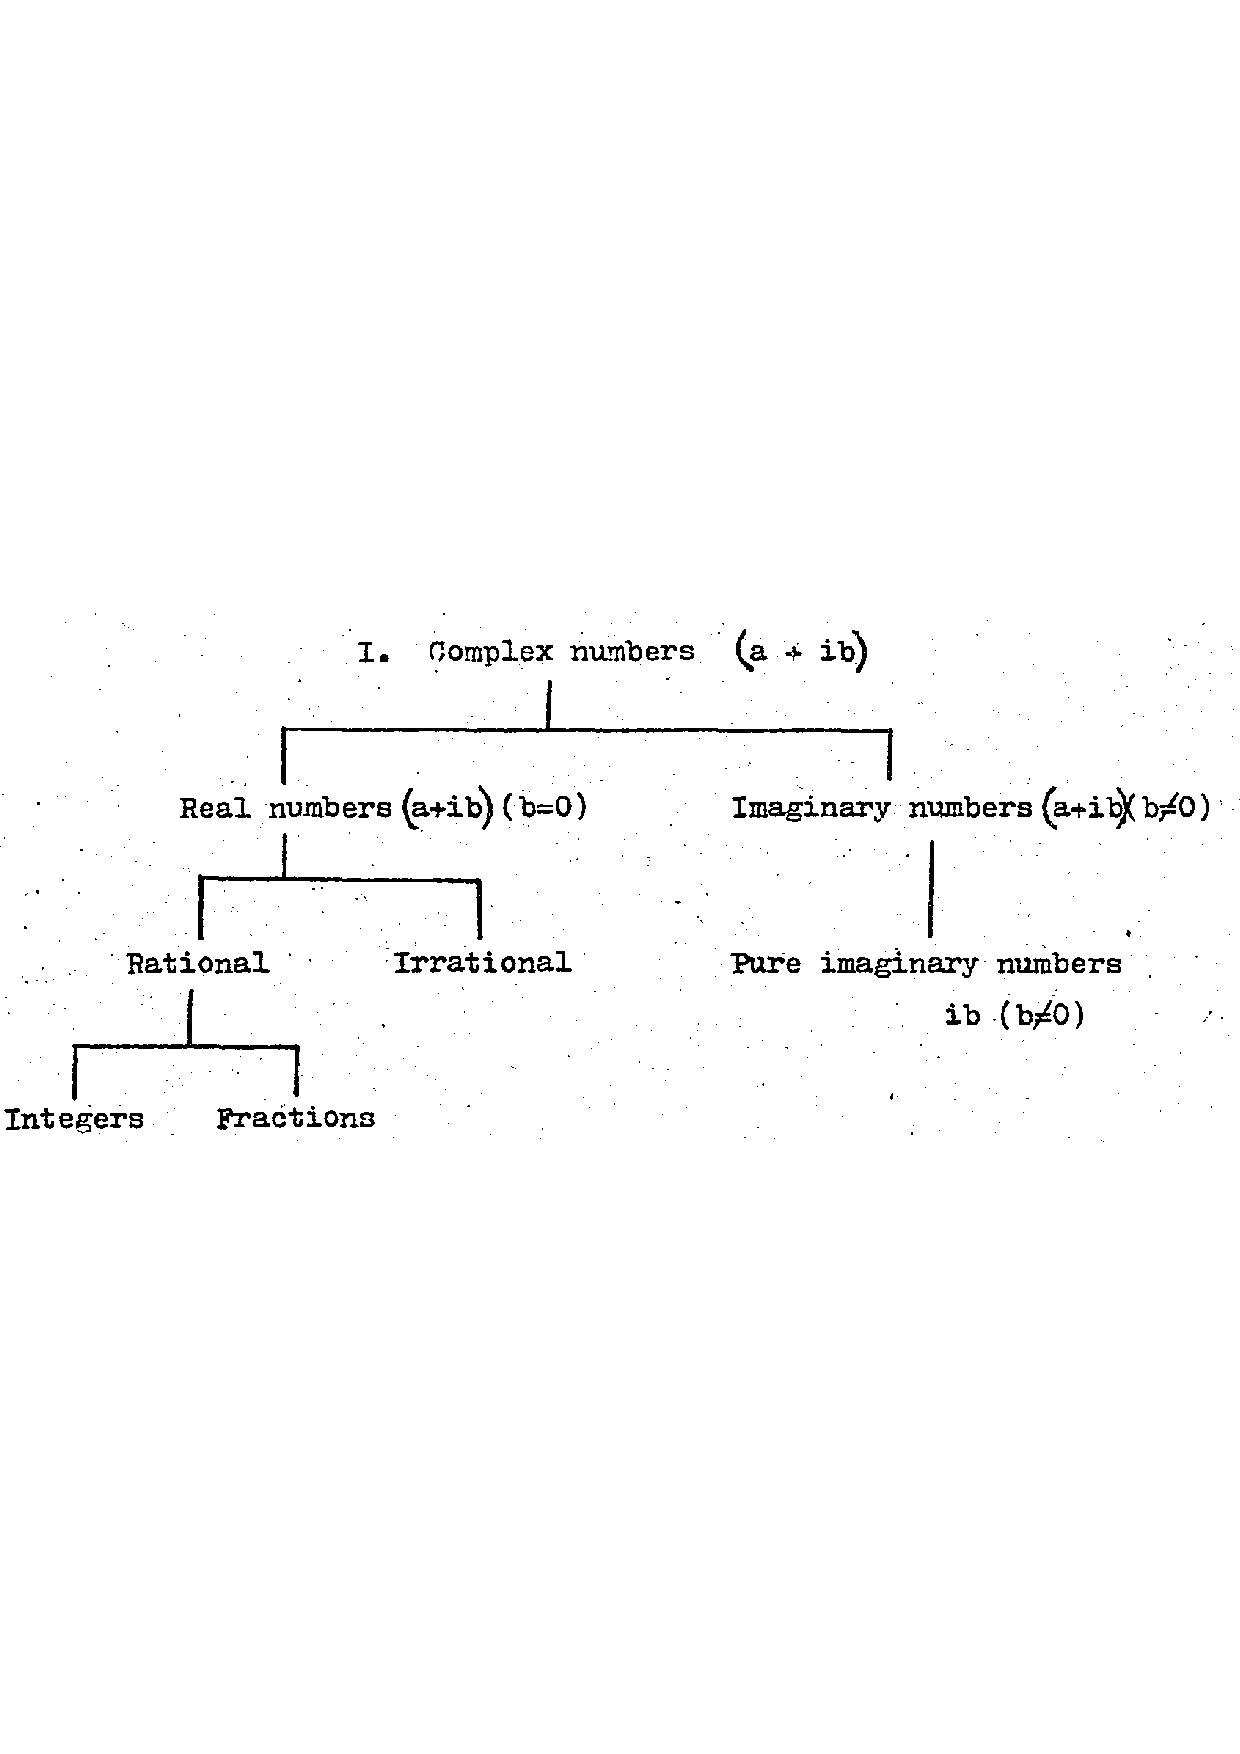
\includegraphics[width=0.9\textwidth]{images/SD-1-1p15A}
%	\caption{Classification of complex numbers}
%	\label{fig:classificationOfComplexNumbersA}
%\end{figure}

%\begin{center}
%\begin{tabular}{cc}
%\end{tabular}
%\end{center}

%\begin{exmp}
%\begin{hSolution}
%\end{hSolution}
%\end{exmp}

%\begin{hEnumerateAlpha}
%\end{hEnumerateAlpha}

%\begin{hEnumerateRoman}
%\end{hEnumerateRoman}

%$
%\begin{bmatrix}
%\end{bmatrix}
%$

%\frac{aaaa}{bbb}
%\frac{a_{n}}{b_{n}}
%\left( aaaa \right)
%\Longrightarrow

%\begin{multicols}{2}
%	bb
%\columnbreak
%	aa
%\end{multicols}
